\documentclass{standalone}
\usepackage{tikz}
\usetikzlibrary{shapes, arrows.meta, positioning, calc}

\begin{document}
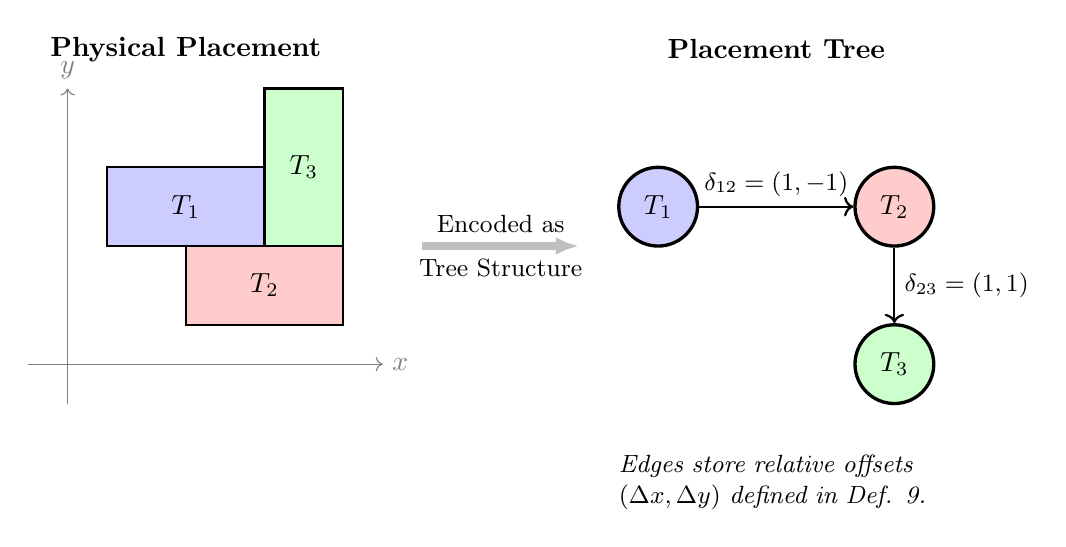
\begin{tikzpicture}[
    node distance=2cm,
    stringNode/.style={circle, draw=black, fill=white, very thick, minimum size=1cm},
    gridBox/.style={rectangle, draw=gray, dashed, minimum width=0.8cm, minimum height=0.6cm}
]

    % --- LEFT PANEL: PHYSICAL PLACEMENT ---
    \node[font=\bfseries] at (1.5, 4) {Physical Placement};
    
    % Coordinate System axes
    \draw[->, gray] (-0.5,0) -- (4,0) node[right] {$x$};
    \draw[->, gray] (0,-0.5) -- (0,3.5) node[above] {$y$};
    
    % String T1 (Root)
    \draw[fill=blue!20, thick] (0.5, 1.5) rectangle (2.5, 2.5);
    \node at (1.5, 2) {$T_1$};
    
    % String T2 (Offset from T1)
    % Placed relative to T1 by (1, -1)
    \draw[fill=red!20, thick] (1.5, 0.5) rectangle (3.5, 1.5);
    \node at (2.5, 1) {$T_2$};
    
    % String T3 (Offset from T2)
    % Placed relative to T2 by (1, 1)
    \draw[fill=green!20, thick] (2.5, 1.5) rectangle (3.5, 3.5);
    \node at (3, 2.5) {$T_3$};

    % --- SEPARATOR ARROW ---
    \draw[-{Latex[length=3mm]}, line width=1mm, gray!50] (4.5, 1.5) -- (6.5, 1.5) 
        node[midway, above, text=black, font=\small] {Encoded as}
        node[midway, below, text=black, font=\small] {Tree Structure};

    % --- RIGHT PANEL: PLACEMENT TREE ---
    \node[font=\bfseries] at (9, 4) {Placement Tree};

    % Tree Nodes
    \node[stringNode, fill=blue!20] (n1) at (7.5, 2) {$T_1$};
    \node[stringNode, fill=red!20] (n2) at (10.5, 2) {$T_2$};
    \node[stringNode, fill=green!20] (n3) at (10.5, 0) {$T_3$};

    % Tree Edges with Offsets
    % Edge T1 -> T2
    \draw[->, thick] (n1) -- (n2) 
        node[midway, above, font=\small] {$\delta_{12} = (1, -1)$};
        
    % Edge T2 -> T3
    \draw[->, thick] (n2) -- (n3)
        node[midway, right, font=\small] {$\delta_{23} = (1, 1)$};

    % Annotation
    \node[align=left, font=\small, text width=4cm] at (9, -1.5) {
        \textit{Edges store relative offsets $(\Delta x, \Delta y)$ defined in Def. 9.}
    };

\end{tikzpicture}

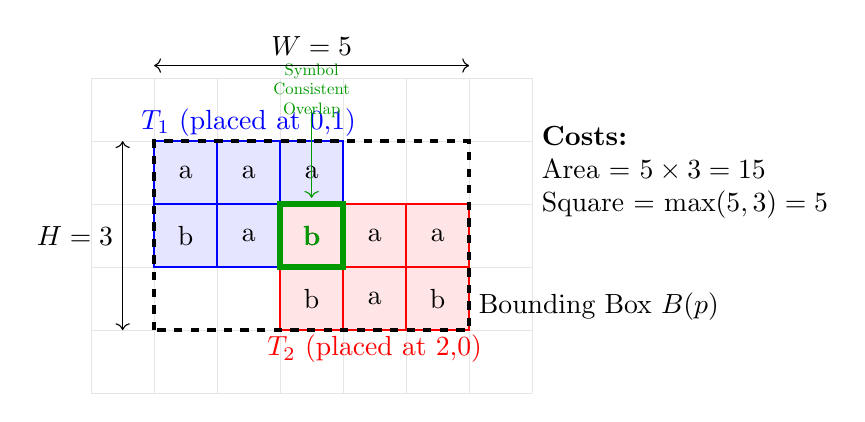
\begin{tikzpicture}[scale=0.8]
    % Grid
    \draw[step=1cm,gray!20,very thin] (-1,-1) grid (6,4);

    % String T1 (Blue) at (0,1) size 3x2
    \fill[blue!10] (0,1) rectangle (3,3);
    \draw[blue, thick] (0,1) grid (3,3);
    \draw[blue, thick] (0,1) rectangle (3,3);
    \node[blue] at (1.5, 3.3) {$T_1$ (placed at 0,1)};
    % Symbols for T1
    \node at (0.5,1.5) {b}; \node at (1.5,1.5) {a}; \node at (2.5,1.5) {b};
    \node at (0.5,2.5) {a}; \node at (1.5,2.5) {a}; \node at (2.5,2.5) {a};

    % String T2 (Red) at (2,0) size 3x2
    \fill[red!10] (2,0) rectangle (5,2);
    \draw[red, thick] (2,0) grid (5,2);
    \draw[red, thick] (2,0) rectangle (5,2);
    \node[red] at (3.5, -0.3) {$T_2$ (placed at 2,0)};
    % Symbols for T2
    \node at (2.5,0.5) {b}; \node at (3.5,0.5) {a}; \node at (4.5,0.5) {b};
    \node at (2.5,1.5) {b}; \node at (3.5,1.5) {a}; \node at (4.5,1.5) {a};

    % Intersection Highlight
    \draw[green!60!black, line width=2pt] (2,1) rectangle (3,2);
    \node[green!60!black, font=\bfseries] at (2.5,1.5) {b};
    \node[green!60!black, scale=0.6, align=center] at (2.5, 3.8) {Symbol\\Consistent\\Overlap};
    \draw[->, green!60!black] (2.5, 3.5) -- (2.5, 2.1);

    % Bounding Box
    \draw[dashed, ultra thick, black] (0,0) rectangle (5,3);
    \node[anchor=south west] at (5,0) {Bounding Box $B(p)$};
    
    % Dimensions
    \draw[<->] (-0.5,0) -- (-0.5,3) node[midway, left] {$H=3$};
    \draw[<->] (0,4.2) -- (5,4.2) node[midway, above] {$W=5$};

    % Cost Text
    \node[align=left, anchor=west] at (6,2.5) {\textbf{Costs:}\\ Area = $5 \times 3 = 15$\\ Square = $\max(5,3) = 5$};

\end{tikzpicture}



% \begin{tikzpicture}[
%     scale=0.8,
%     cell/.style={draw, minimum size=1cm, anchor=center, font=\sffamily\Large},
%     stringA/.style={fill=blue!10},
%     stringB/.style={fill=red!10},
%     overlap/.style={fill=purple!20, pattern=north east lines, pattern color=purple}
% ]

%     % --- Grid Background (Optional) ---
%     \draw[step=1cm, gray!20, very thin] (-1,-1) grid (5,4);

%     % --- String 1: "a b a / b a b" placed at (0,1) ---
%     % Coordinates are (x,y)
%     \node[cell, stringA] at (0.5, 2.5) {a};
%     \node[cell, stringA] at (1.5, 2.5) {b};
%     \node[cell, stringA] at (2.5, 2.5) {a};
%     \node[cell, stringA] at (0.5, 1.5) {b};
%     \node[cell, stringA] at (1.5, 1.5) {a};
%     \node[cell, stringA] at (2.5, 1.5) {b};
    
%     % Label for String 1
%     \node[blue!80, font=\bfseries] at (0.5, 3.2) {$T_1$};

%     % --- String 2: "a b / a b" placed at (2,0) ---
%     % Notice (2,1) and (2,2) are overlaps
    
%     % Non-overlapping part of T2
%     \node[cell, stringB] at (3.5, 1.5) {a};
%     \node[cell, stringB] at (3.5, 0.5) {b};
%     \node[cell, stringB] at (2.5, 0.5) {a};

%     % Overlapping part (Symbol Consistent)
%     % Overlaps with T1 at x=2, y=1 and y=2? 
%     % Let's make T2 be 2x2 matrix: "b a / a b"
%     % Overlap at (2,1) which is 'b' in T1. So T2 must have 'b' there.
%     \node[cell, overlap] at (2.5, 1.5) {b}; % Overlap cell
    
%     % Label for String 2
%     \node[red!80, font=\bfseries] at (3.5, -0.2) {$T_2$};

%     % --- Bounding Box ---
%     % Bounding box covers x=0 to 4, y=0 to 3
%     \draw[dashed, thick, black!80] (0,0) rectangle (4,3);
    
%     % Dimensions lines
%     \draw[<->] (0, -0.7) -- (4, -0.7) node[midway, below] {Width $W=4$};
%     \draw[<->] (-0.7, 0) -- (-0.7, 3) node[midway, left, rotate=90] {Height $H=3$};
    
%     % Objective Function text
%     \node[align=left, font=\small] at (6, 1.5) {
%         \textbf{Objective:}\\
%         Minimize Area $= W \times H$\\
%         $= 12$\\
%         \textit{(Includes empty cells)}
%     };

% \end{tikzpicture}

\end{document}